% Basic stuff
\documentclass[a4paper,10pt]{article}
\usepackage[utf8]{inputenc}
\usepackage[T1]{fontenc}
\usepackage[nswissgerman]{babel}
\usepackage{gensymb}
\usepackage{multicol}
\usepackage{float}
\usepackage{pgfplots}
\pgfplotsset{compat=newest}


\usepackage{zref-totpages}
\makeatletter
\renewcommand{\@evenfoot}{\hfil \thepage{}/\ztotpages\hfil}
\renewcommand{\@oddfoot}{\@evenfoot}
\makeatother

% 3 column landscape layout with fewer margins
\usepackage[landscape, left=0.75cm, top=1cm, right=0.75cm, bottom=1.5cm, footskip=15pt]{geometry}
\usepackage{flowfram}
\ffvadjustfalse
\setlength{\columnsep}{1cm}
\Ncolumn{3}

% define nice looking boxes
\usepackage[many]{tcolorbox}

% a base set, that is then customised

\tcbset {
  base/.style={
    boxrule=0mm,
    leftrule=0mm,
    left=1.75mm,
    arc=1mm, 
    fonttitle=\bfseries, 
    colbacktitle=black!10!white, 
    coltitle=black, 
    toptitle=0.75mm, 
    bottomtitle=0.25mm,
    title={#1}
  }
}

\definecolor{bluetitle}{RGB}{210, 235, 255}
\definecolor{blueframe}{RGB}{146, 208, 255}
\definecolor{blueback}{RGB}{236, 247, 255}
\newtcolorbox{mainbox}[1]{
  colframe=blueframe, 
  base={#1},
  colbacktitle=bluetitle,
  colback=blueback,
}

\newtcolorbox{subbox}[1]{
  colframe=black!20!white,
  base={#1}
}

% Mathematical typesetting & symbols
\usepackage{amsthm, mathtools, amssymb} 
\usepackage{marvosym, wasysym}
\allowdisplaybreaks

% Tables
\usepackage{tabularx, multirow}
\usepackage{booktabs}
\renewcommand*{\arraystretch}{2}

% Make enumerations more compact
\usepackage{enumitem}
\setitemize{itemsep=0.5pt}
\setenumerate{itemsep=0.75pt}

% To include sketches & PDFs
\usepackage{graphicx}

% For hyperlinks
\usepackage{hyperref}
\hypersetup{
  colorlinks=true
}

% Metadata
\title{Analysis I}
\author{by Silvan Metzker}
\date{June 2023}

% Math helper stuff
\def\limn{\lim_{n\to \infty}}
\def\limxo{\lim_{x\to 0}}
\def\limxi{\lim_{x\to\infty}}
\def\limxn{\lim_{x\to-\infty}}
\def\sumk{\sum_{k=1}^\infty}
\def\sumn{\sum_{n=0}^\infty}
\def\R{\mathbb{R}}
\def\dx{\text{ d}x}

\begin{document}

\setlength{\abovedisplayskip}{3pt}
\setlength{\belowdisplayskip}{3pt}
\setlength{\abovedisplayshortskip}{3pt}
\setlength{\belowdisplayshortskip}{3pt}

\begin{center}
	\vspace{1cm}
	{\Large \textsc{Cheat Sheet}\par}
	{\huge\bfseries Analysis I\par}
	\vspace{0.5cm}
	{\Large\itshape Silvan Metzker\par}
	{\large Juni 2023\par}
	\vspace{0.4cm}
	{\textbf{Lizenz:} CC BY-SA 4.0}
\end{center}

\section{Reelle \& Komplexe Zahlen}
\subsection{Reelle Zahlen}
$\R$ ist ein kommutativer, angeordneter Körper, der ordnungsvollständig ist.

\begin{mainbox}{Axiome der Addition}
	\textbf{A1} Assoziativität \\$x + (y + z) = (x + y) + z \; \forall x,y,z \in \R$ \\ \\
	\textbf{A2} Neutrales Element \\$x + 0 = x \; \forall x \in \R$ \\ \\
	\textbf{A3} Inverses Element \\$\forall x \in \R \; \exists y \in \R : x + y = 0$ \\ \\
	\textbf{A4} Kommutativität \\$x + z = z + x \; \forall x, z \in \R$
\end{mainbox}

\begin{mainbox}{Axiome der Multiplikation}
	\textbf{M1} Assoziativität\\ $x \cdot (y \cdot z) = (x \cdot y) \cdot z \; \forall x,y,z \in \R$\\\\
	\textbf{M2} Neutrales Element\\ $x \cdot 1 = x \; \forall x \in \R$ \\\\
	\textbf{M3} Inverses Element\\ $\forall x \in \R \backslash \{0\} \; \exists y \in \R : x \cdot y = 1$ \\\\
	\textbf{M4} Kommutativität\\ $x \cdot z = z \cdot x \; \forall x, z \in \R$
\end{mainbox}

D Distributivität $x \cdot (y + z) = x \cdot y + x \cdot z \; \forall x,y,z \in \R$

\begin{mainbox}{Ordnugsaxiome}
	\textbf{O1} Reflexivität \\$x \leqslant x \; \forall x \in \R$ \\\\
	\textbf{O2} Transitivität \\$x \leqslant y$ und $y \leqslant z \Longrightarrow x \leqslant z$ \\\\
	\textbf{O3} Antisymmetrie \\$x \leqslant y$ und $y \leqslant x \Longrightarrow x = y$ \\\\
	\textbf{O4} Total \\$ \forall x, y \in \R$ gilt entweder $x \leqslant y$ oder $y \leqslant x$
\end{mainbox}

\begin{subbox}{Kompatibilität}
	\textbf{K1} $\forall x,y,z \in \R : x \leqslant y \Longrightarrow x + z \leqslant y + z$ \\
	\textbf{K2} $ \forall x \geqslant 0, \; \forall y \geqslant 0 : x \cdot y \geqslant 0$
\end{subbox}

	
\begin{mainbox}{Ordnungsvollständigkeit}
	Sein $A$, $B$ Teilmengen von $\R$, so dass
	\begin{itemize}
		\item[i)] $A \neq \emptyset$, $B \neq \emptyset$
		\item[ii)] $\forall a \in A$ und $\forall b \in B$ gilt: $a \leqslant b$
	\end{itemize}
	Dann gibt es $c \in \R$, so dass $\forall a \in A : a \leqslant c$ und $\forall b \in B : c \leqslant b$
\end{mainbox}

\subsubsection*{Archimedisches Prinzip}
Sei $x < \in \R$ mit $x > 0$ und $y \in \R$. Dann gibt es $n \in \mathbb{N}$ mit $y \leqslant n \cdot x$. \\


\begin{center}
	\tikzset{every picture/.style={line width=0.75pt}} %set default line width to 0.75pt        
	
	\begin{tikzpicture}[x=0.75pt,y=0.75pt,yscale=-1,xscale=1]
		%uncomment if require: \path (0,112); %set diagram left start at 0, and has height of 112
		
		%Straight Lines [id:da7469803271598898] 
		\draw [line width=1.5]    (0.33,25.64) -- (51.81,25.64) -- (266.9,25.64) ;
		%Straight Lines [id:da6811773464337398] 
		\draw [line width=1.5]    (19.33,14.61) -- (19.33,36.67) ;
		%Straight Lines [id:da6645341706273629] 
		\draw [line width=1.5]    (75.09,14.61) -- (75.09,36.67) ;
		%Straight Lines [id:da43913292143899507] 
		\draw [line width=1.5]    (130.25,14.61) -- (130.25,36.67) ;
		%Straight Lines [id:da5331078132500611] 
		\draw [line width=1.5]    (185.4,14.61) -- (185.4,36.67) ;
		%Straight Lines [id:da953154069584746] 
		\draw [line width=1.5]    (240.55,14.61) -- (240.55,36.67) ;
		%Straight Lines [id:da02282522199409287] 
		\draw [color={rgb, 255:red, 74; green, 144; blue, 226 }  ,draw opacity=1 ][line width=1.5]    (197.04,14.61) -- (197.04,36.67) ;
		
		% Text Node
		\draw (14.23,41.53) node [anchor=north west][inner sep=0.75pt]  [font=\normalsize] [align=left] {$0$};
		% Text Node
		\draw (70.33,45.25) node [anchor=north west][inner sep=0.75pt]  [font=\normalsize] [align=left] {$x$};
		% Text Node
		\draw (121.53,41.53) node [anchor=north west][inner sep=0.75pt]  [font=\normalsize] [align=left] {$2x$};
		% Text Node
		\draw (176.96,42.81) node [anchor=north west][inner sep=0.75pt]  [font=\normalsize] [align=left] {$3x$};
		% Text Node
		\draw (232.16,42.2) node [anchor=north west][inner sep=0.75pt]  [font=\normalsize] [align=left] {$4x$};
		% Text Node
		\draw (192.66,2.53) node [anchor=north west][inner sep=0.75pt]  [font=\normalsize] [align=left] {$y$};
		
		
	\end{tikzpicture}
	
\end{center}

\subsubsection*{Beschränktheit}
$A \in \R$ heisst von oben/unten beschränkt (v.o.b/v.u.b), falls es ein $x \in \R$ gibt, so dass $x \geqslant a$/$x \leqslant a$ für $\forall a \in A$. $x$ ist dann die obere/untere Schranke und A ist v.o.b/v.u.b. Falls $x \in A$ ist und $x$ eine obere/untere Schranke ist, heisst es Maximum/minimum von $A$.

\begin{mainbox}{Rechnen mit Absolutbeträgen}
	Für alle $x,y \in \mathbb{R}$ gilt:
	\begin{multicols}{2}
		\begin{itemize}
			\item[i)] $|x|\geq 0$
			\item[ii)] $|xy|=|x||y|$
			\item[iii)] $|x+y|\leq |x|+|y|$
			\item[iv)] $|x+y|\geq||x|-|y||$
		\end{itemize}
	\end{multicols}
\end{mainbox}

\begin{mainbox}{Supremum \& Infimum}
	Sei $A \in \R$, $A \neq \emptyset$
	\begin{itemize}
		\item[i)] Ist $A$ v.o.b, dann gibt es eine kleinste obere Schranke $c := \sup A$, das Supremum von A.
		\item[ii)] Ist $A$ v.u.b, dann gibt es eine grösste untere Schranke $d := \inf A$, das Infimum von A.
	\end{itemize}
\end{mainbox}
\subsection{Komplexe Zahlen}
\begin{mainbox}{Konjugation}
	\centerline{$z = x + iy \in \mathbb{C} \qquad\longrightarrow\qquad \overline{z} = x - iy \in \mathbb{C}\\$}
	\vspace{10pt}
	Die Konjugation hat die folgenden Eigenschaften
	\begin{itemize}
		\item[i)]  $z \cdot \overline{z} = (x + iy) \cdot (x - iy) = x^2 - i^2 \cdot y^2 \\ = x^2 + y^2 = |z|^2 \Longrightarrow z^{-1} = \frac{\overline{z}}{|z|^2}$, $z \neq 0$
		\item[ii)] $\overline{(z_1 + z_2)} = \overline{z_1} + \overline{z_2}$
		\item[iii)] $\overline{(z_i \cdot z_2)} = \overline{z_1} \cdot \overline{z_2}$
	\end{itemize}
\end{mainbox}
\begin{mainbox}{Reel- und Imaginärteil}
	Für jedes $z\in\mathbb{Z}$ gilt:
	$$
	\operatorname{Re}(z)=\frac{z+\bar{z}}{2} \qquad \operatorname{Im}(z)=\frac{z-\bar{z}}{2i} \qquad
	$$	
	Und es gilt:
	$$z\in\mathbb{R}\Longleftrightarrow z = \bar{z}$$
	
\end{mainbox}


\begin{mainbox}{Polarform}
	Die Polarform von $z = x + iy \in \mathbb{C}$ ($\phi \in (- \pi, \pi]$) 
	\begin{align*}
		z                                     & = r \cdot e^{i \cdot \pi}                                       \\
		z                                     & = r \cdot (\cos(\phi) + i \cdot \sin(\phi))\text{, mit }r = |z| \\
		|z|                                   & = \sqrt{x^2 + y^2}\qquad |z|^2 = x^2+y^2                        \\
		x                                     & = r \cdot \cos(\phi),                                           \\
		y                                     & = r \cdot \sin(\phi)                                            \\
		\phi                                  & =                                                               
		\begin{cases}
		\arctan\left(\frac{y}{x}\right)       & x > 0                                                           \\
		\arctan\left(\frac{y}{x}\right) + \pi & x < 0 \land y \geqslant 0                                       \\
		\arctan\left(\frac{y}{x}\right) - \pi & x < 0 \land y < 0                                               \\
		\frac{\pi}{2}                         & x = 0  \land y > 0                                              \\
		- \frac{\pi}{2}                       & x = 0 \land y < 0                                               \\
		\text{undefiniert}                    & x = 0 \land y = 0                                               \\
		\end{cases}
		\
	\end{align*}
	  
\end{mainbox}

\begin{mainbox}{Fundamentalsatz der Algebra}
	Sei $n\geq 1, n\in \mathbb{N}$ und\\ 
	\centerline{$\operatorname{P}(z)=z^n+a_{n-1}z^{n-1}+\dots+a_0, \qquad a_i\in \mathbb{C}$}\\
	Dann gibt es $z_1,\dots,z_n \in \mathbb{C}$, so dass\\
	\centerline{$\operatorname{P}(z)=(z-z_1)(z-z_2)\cdot \dotsc \cdot (z-z_n$)}
\end{mainbox}

\section{Folgen}
\subsection{Konvergenz}
Eine Folge $(a_n)_{n\in \mathbb{N}}$ heisst \textbf{konvergent}, falls es $l \in \mathbb{R}$ gibt, sodass $\forall \varepsilon > 0$ die folgende Menge endlich ist: \\
\centerline{$\{n\in\mathbb{N}^* \mid a_n\notin \ ]l - \varepsilon,l - \varepsilon[\}$ }\\
Eine Folge $(a_n)_{n\in \mathbb{N}}$ konvergiert gegen $L$ (oder Funktion)\\ $\iff \lim_{n \to \infty} a_n = L $ \\ $\iff \forall \varepsilon > 0 \ \exists N_\varepsilon \ \forall n \ge N_\varepsilon : \ | a_n - L | < \varepsilon$\\

Wir dürfen (o.B.d.A.) annehmen, dass $\varepsilon$ durch eine Konstante $C \in \R$ beschränkt ist.
Es gilt ausserdem:
\begin{itemize}
	\item konvergent $\implies$ beschränkt, aber nicht umgekehrt
	\item $(a_n)$ konvergent $\iff (a_n)$ beschränkt \textbf{und} \\$\lim \inf a_n = \lim \sup a_n$
\end{itemize}


\begin{subbox}{Limes Superior \& Inferior}
	$\limn \inf x_n = \limn \left( \inf_{m \ge n} x_m \right)$ \\
	$\limn \sup x_n = \limn \left( \sup_{m \ge n} x_m \right)$
\end{subbox}

\begin{mainbox}{Einschliessungskriterium \\ (Sandwich-Theorem)}
	Wenn $\limn a_n = \alpha, \ \limn b_n = \alpha$ und $a_n \le c_n \le b_n, \forall n \ge k$, dann $\limn c_n = \alpha$.
\end{mainbox}

\begin{mainbox}{Weierstrass}
	Wenn $a_n$ monoton wachsend und nach oben beschränkt ist, dann konvergiert $a_n$ mit Grenzwert $\limn a_n = \sup \{a_n : \ n \ge 1\}$.
	
	Wenn $a_n$ monoton fallend und nach unten beschränkt ist, dann konvergiert $a_n$ mit Grenzwert $\limn a_n = \inf \{a_n : \ n \ge 1\}$.
\end{mainbox}

\begin{subbox}{Limes von Folgen}
	Seien $(a_n)_{n\geq 1}$ und 	$(b_n)_{n\geq 1}$ konvergente Folgen mit $a=\lim_{n\rightarrow\infty} a_n$ und $b=\lim_{n\rightarrow\infty} b_n$.
	\begin{itemize}[leftmargin=18pt]
		\item[i)] $(a_n+b_n)_{n\geq 1}$ konv. und $\lim_{n\rightarrow\infty} (a_n+b_n)= a+b$.
		\item[ii)] $(a_n\cdot b_n)_{n\geq 1}$ konv. und $\lim_{n\rightarrow\infty} (a_n\cdot b_n)= a \cdot b$.
		\item[iii)] Wenn $b_i \neq 0$ und $b \neq 0$ \hfill($\forall i\geq 1$)
		      \\$(a_n / b_n)_{n\geq 1}$ konv. und $\lim_{n\rightarrow\infty} (a_n / b_n)= a / b$.
		\item[iv)] Wenn $\exists K \geq 1$ mit $a_n \leq^* b_n, \forall n\geq K$\\
		      $\Rightarrow a \leq^* b$\hfill ($^*$ funktioniert nicht mit ``$<$'')
	\end{itemize}
\end{subbox}


\begin{mainbox}{Cauchy-Kriterium}
	Die Folge $a_n$ ist genau dann konvergent, falls $\\\forall \varepsilon > 0 \ \exists N \ge 1$ so dass $| a_n - a_m | < \varepsilon \hfill \forall n,m \ge N$.
\end{mainbox}

\begin{subbox}{Monoton Fallend/Wachsend}
	Die Folge $(a_n)_{n\geq 1}$	ist monoton fallend/wachsend, wenn $\forall n\geq 1$ gilt $a_n \geq a_{n+1}$/$a_n \leq a_{n+1}$.
\end{subbox}


\subsubsection{Teilfolge}
Eine Teilfolge von $a_n$ ist eine Folge $b_n$ wobei $b_n = a_{l(n)}$ und $l$ eine Funktion mit $l(n) < l(n+1) \quad \forall n \ge 1$ (z.B. $l = 2n$ für jedes gerade Folgenglied). 

\subsubsection{Bolzano-Weierstrass}
Jede beschränkte Folge besitzt eine konvergente Teilfolge.

\subsection{Strategie - Konvergenz von Folgen}
\begin{enumerate}
	\item Bei Brüchen: Grösste Potenz von $n$ kürzen. Alle Brüche der Form $\frac{a}{n^a}$ streichen, da diese nach 0 gehen.
	\item Bei Wurzeln in Summe im Nenner: Multiplizieren des Nenners und Zählers mit der Differenz der Summe im Nenner. (z.B. $(a+b)$ mit $(a-b)$ multiplizieren)
	\item Bei rekursiven Folgen: Anwendung von Weierstrass zur monotonen Konvergenz
	\item Einschliessungskriterium (Sandwich-Theorem) anwenden.
	\item Mit bekannter Folge vergleichen.
	\item Grenzwert durch einfaches Umformen ermitteln.
	\item Limit per Definition der Konvergenz zeigen.
	\item Anwendung des Cauchy-Kriteriums.
	\item Suchen eines konvergenten Majorant.
	\item Weinen und die Aufgabe überspringen.
\end{enumerate}

\subsection{Strategie - Divergenz von Folgen}
\begin{enumerate}
	\item Suchen einer divergenten Vergleichsfolge.
	\item Alternierende Folgen: Zeige, dass Teilfolgen nicht gleich werden, also $\limn a_{p_1(n)} \ne \limn a_{p_2(n)}$ (mit z.B. gerade/ungerade als Teilfolgen).
\end{enumerate}

\newpage
\subsection{Tricks für Grenzwerte}
\subsubsection{Binome}
$$\lim_{x\to\infty} (\sqrt{x + 4} - \sqrt{x - 2}) = \lim_{x\to\infty} \frac{(x+4)-(x-2)}{\sqrt{x+4}+\sqrt{x-2}}$$

\subsubsection{Substitution}
$$\lim_{x\to\infty} x^2 \left(1-\cos\left(\frac{1}{x}\right)\right)$$
Substituiere nun $u = \frac{1}{x}$:
$$\lim_{u \to 0} \frac{1 - \cos(u)}{u^2} = \lim_{u \to 0} \frac{\sin(u)}{2u} = \lim_{u\to 0} \frac{\cos(u)}{2} = \frac{1}{2}$$

\subsubsection{Induktive Folgen (Induktionstrick)}
\begin{enumerate}
	\item Zeige monoton wachsend / fallend
	\item Zeige beschränkt
	\item Nutze Satz von Weierstrass, d.h. Folge muss gegen Grenzwert konvergieren
	\item Verwende Induktionstrick:
\end{enumerate}
Wenn die Folge konvergiert, hat jede Teilfolge den gleichen Grenzwert. Betrachte die Teilfolge $l(n) = n + 1$ für $d_{n+1} = \sqrt{3d_n - 2}$:
$$d = \lim_{n\to\infty} d_n = \lim_{n\to\infty} d_{n+1} = \sqrt{\lim_{n \to \infty} 3d_n -2} = \sqrt{3d -2}$$
Forme um zu $ d^2 = 3d -2 \to d \in {1,2}$. Nun können wir $d = 2$ nehmen und die Beschränktheit mit $d=2$ per Induktion zeigen.\\

\begin{subbox}{Wurzel Trick für $\sqrt{n+1}-\sqrt{n}$}
	\begin{align*}
		\sqrt{n+1}-\sqrt{n} & =(\sqrt{n+1}-\sqrt{n})\frac{\sqrt{n+1}+\sqrt{n}}{\sqrt{n+1}+\sqrt{n}}              \\
		                    & =\frac{\sqrt{n+1}^2-\sqrt{n}^2}{\sqrt{n+1}+\sqrt{n}} \qquad \text{(binom. Formel)} \\
		                    & =\frac{1}{\sqrt{n+1}+\sqrt{n}}                                                     
	\end{align*}
\end{subbox}
\section{Reihen}

\begin{mainbox}{Cauchy-Kriterium für Reihen}
	Die Reihe $\sumk a_k$ ist genau dann konvergent, falls 
	\centerline{$\forall \varepsilon > 0 \ \exists N \ge 1$ mit $| \sum_{k=n}^m a_k | < \varepsilon, \ \forall m \ge n \ge N$.}
\end{mainbox}

\begin{subbox}{Nullfolgenkriterium}
	Wenn für eine Folge $\limn |a_n| \ne 0$ ist, dann divergiert $\sumn a_n$.
\end{subbox}


\subsubsection{Reihenarithmetik}
Wenn $\sumk a_k$ und $\sumk b_k$ konvergent sind, dann gilt:
\begin{itemize}
	\item $\sumk (a_k + b_k)$ konvergent und $\sumk (a_k + b_k) = \left( \sumk a_k \right) + \left( \sumk b_k \right)$
	\item $\sumk \alpha a_k$ konvergent und $\sumk \alpha a_k = \alpha \sumk a_k$
\end{itemize}


\begin{mainbox}{Vergleichssatz}
	Wenn $\sumk a_k$ und $\sumk b_k$ Reihen mit $0 \le a_k \le b_k, \forall k \ge K \ge 1$ sind, so gilt:
	$$\sumk b_k \text{ konvergent} \implies \sumk a_k \text{ konvergent}$$ 
	$$\sumk a_k \text{ divergent} \implies \sumk b_k \text{ divergent}$$ 
\end{mainbox}

Als Vergleichsreihe (Majorant / Minorant) eignet sich oft eine Reihe der folgenden Kategorien:
\subsubsection{Geometrische Reihe} 
$\sum_{k=0}^\infty q^k$ divergiert für $|q| \ge 1$ und konvergiert zu $\frac{1}{1 - q}$ für $|q| < 1$
\subsubsection{Zeta-Funktion}
$\zeta(s) = \sum_{n=1}^\infty \frac{1}{n^s}$ divergiert für $s \le 1$ und konvergiert für $s > 1$.

\subsection{Absolute Konvergenz}
$\sumk a_k$ heisst \textbf{absolut konvergent}, wenn $\sumk |a_k|$ konvergiert. Eine absolut konvergente Reihe ist immer auch konvergent, es gilt $|\sumk a_k| \le \sumk |a_k|$.

Falls eine Reihe absolut konvergiert, dann konvergiert jede Umordnung der Reihe mit dem selben Grenzwert.

\noindent Ansonsten gibt es immer eine Anordnung, so dass \\
\centerline{$\sum_{k=1}^\infty a_{\phi(k)} = x, \ \forall x\in \R$.}

\begin{subbox}{Leibnizkriterium}
	Wenn $a_n \ge 0, \ \forall n \ge 1$ monoton fallend ist und $\limn a_n = 0$ gilt, dann konvergiert \\
	\centerline{$S = \sumk (-1)^{k+1} a_k$ \textit{und} $a_1 - a_2 \le S \le a_1$.}
\end{subbox}

\begin{mainbox}{Quotientenkriterium}
	Sei $(a_n)$ eine Folge mit $a_n \ne 0, \forall n \ge 1$.  
	\begin{align*}
		\textstyle \limn \sup \frac{|a_{n+1}|}{|a_n|} < 1 & \implies \textstyle \sum_{n=1}^\infty a_n \text{ konv. absolut.} \\ 
		\textstyle \limn \inf \frac{|a_{n+1}|}{|a_n|} > 1 & \implies \textstyle \sum_{n=1}^\infty a_n \text{ divergiert.}    
	\end{align*}
	
\end{mainbox}

\begin{mainbox}{Wurzelkriterium}
	Sei $(a_n)$ eine Folge mit $a_n \ne 0, \forall n \ge 1$. Sei $q = \limn \sup \sqrt[n]{|a_n|}$. 
	\begin{itemize}
		\item $q < 1 \implies \sum_{n=1}^\infty a_n$ konvergiert absolut.
		\item $q = 1 \implies$ keine Aussage.
		\item $q > 1 \implies \sum_{n=1}^\infty a_n$ und $\sum_{n=1}^\infty |a_n|$ diverg.
	\end{itemize}
\end{mainbox}

\subsection{Wichtige Reihen}
\begin{table}[H]
	\begin{tabular}{ll}
		$\displaystyle\sum_{i=1}^n i^2 = \frac{1}{6}n(n+1)(2n+1)$ & $\displaystyle\sum_{i=1}^n i^3 = \frac{1}{4}n^2(n+1)^2$          \\
		$\displaystyle\sum_{i=1}^n q^k = \frac{1}{1-q}$           & $\displaystyle\sum_{i=1}^n i = \frac{n(n+1)}{2}$                 \\
		$\displaystyle\sum_{n=1}^\infty \frac{1}{n(n+1)} = 1$     & $\displaystyle\sum_{i=1}^\infty \frac{1}{i^2} = \frac{\pi^2}{6}$ 
	\end{tabular}
\end{table}

\subsection{Cauchy-Produkt}
\begin{subbox}{Definition Cauchy-Produkt}
	Das Cauchy-Produkt von zwei Reihen $\sum_{i = 0}^\infty a_i$ und $\sum_{j = 0}^\infty b_j$ ist definiert als
	$$\sum_{n=0}^\infty \sum_{j=0}^n (a_{n-j} \cdot b_j) = a_0b_0 + (a_0b_1 + a_1b_0) + \ldots$$ Es konvergiert, falls beide Reihen konvergieren.
\end{subbox}

\subsection{Strategie - Konvergenz von Reihen}
\begin{enumerate}
	\item Ist Reihe ein bekannter Typ? (Teleskopieren, Geometrische/Harmonische Reihe, Zetafunktion, ...)
	\item Ist $\limn a_n = 0$? Wenn nein, divergent.
	\item Quotientenkriterium \& Wurzelkriterium anwenden
	\item Vergleichssatz anwenden, Vergleichsreihen suchen
	\item Leibnizkriterium anwenden
	\item Integral-Test anwenden (Reihe zu Integral)
\end{enumerate}

\subsection{Potenzreihen}
\begin{subbox}{Definition Potenzreihe}
	Potenzreihen sind Reihen der Form:
	$$\sum_{n=0}^\infty a_n x^n$$
	 
	Eine Potenzreihe mit Entwicklungspunkt $x_0$ wird definiert als 
	$$\sum_{n=0}^\infty a_n(x-x_0)^n$$
	 
	Potenzreihen verhalten sich wie folgt:
	$$
	\sum_{n=0}^\infty a_n x^n\begin{cases}
	\text{konvergiert absolut} &|x| < r\\
	\text{divergiert} &|x| > r\\
	\text{keine Aussage} &|x| = r
	\end{cases}
	$$
	Die Variable $r$ ist hierbei der Konvergenzradius.
\end{subbox}

\begin{mainbox}{Konvergenzradius}
	Der Konvergenzradius einer Potenzreihe um einen Entwicklungspunkt $x_0$ ist die grösste Zahl $r$, so dass die Potenzreihe für alle $x$ mit $|x - x_0| < r$ konvergiert. Falls die Reihe für alle $x$ konvergiert, ist der Konvergenzradius $r$ unendlich. Sonst:
	$$r = \limn \left| \frac{a_n}{a_{n+1}} \right| = \frac{1}{\limn\sup \sqrt[n]{|a_n|}} $$
\end{mainbox}



\subsubsection{Definitionen per Potenzreihen}
\begin{align*}
	\exp(x)    & = \sumn \frac{x^n}{n!}                      & r & = \infty \\
	\sin(x)    & = \sumn (-1)^n \frac{x^{2n + 1}}{(2n + 1)!} & r & = \infty \\
	\cos(x)    & = \sumn (-1)^n \frac{x^{2n}}{(2n)!}         & r & = \infty \\
	\ln(x + 1) & = \sumk (-1)^{k+1} \frac{x^k}{k}            & r & = 1      
\end{align*}


\section{Funktionen}
\subsection{Stetigkeit}
Sei $f : D \to \R^d, x \to f(x)$ eine Funktion in $D \subseteq \R^d$.
\begin{mainbox}{Definition Stetigkeit}
	$f$ ist in $x_0 \in D$ stetig, falls $\lim_{x\to x_0} f(x) = f(x_0)$.
	$f$ ist stetig, falls sie in jedem $x_0 \in D$ stetig ist.
	 
	Also falls es für jedes $\varepsilon>0$ ein $\delta>0$ gibt, dass
	\centerline{$|x-x_0|<\delta \Rightarrow |f(x) - f(x_0)|<\varepsilon$}
\end{mainbox}
Polynomiale Funktionen sind auf $\R$ stetig.
\begin{subbox}{}
	Falls $f$ und $g$ den gleichen Definitions-/Bildbereich haben und in $x_0$ stetig sind, dann sind auch $$f + g, \lambda \cdot f, f \cdot g, \frac{f}{g}, |f|, \max(f,g), \min(f,g)$$ stetig in $x_0$.
\end{subbox}


\begin{mainbox}{Zwischenwertsatz}
	Wenn $I \subseteq \R$ ein Intervall, $f: I \to \R$ und $a, b \in I$ ist, dann gibt es für jedes $c$ zwischen $f(a)$ und $f(b)$ ein $a \le z \le b$ mit $f(z) = c$.
	\begin{center}
		\begin{tikzpicture}[domain=0.1:5, samples=100]
			  
			\draw[dashed] (2.9,1.12) -- (-0.2,1.12) node[left] {$f(a)$};
			\draw[dashed] (2.9,1.12) -- (2.9,-0.2) node[below, text height=0.5em] {$a$};
			\draw[dashed] (4.52,1.6) -- (-0.2,1.6) node[left] {$c$};
			\draw[dashed] (4.52,1.6) -- (4.52,-0.2) node[below, text height=0.5em] {$z$};
			\draw[dashed] (4.87,2.5) -- (-0.2,2.5) node[left] {$f(b)$};
			\draw[dashed] (4.87,2.5) -- (4.87,-0.2) node[below, text height=0.5em] {$b$};
			\draw[->, line width=0.3mm] (-0.8,0) -- (6,0) node[right] {$x$};
			\draw[->, line width=0.3mm] (0,-0.5) -- (0,3.5) node[above] {$f(x)$};
			
			\draw[line width=0.3mm, color=black]    plot (\x,{0.25*(\x-1.5)^(3)-0.8*(\x-1.5)^(2)+2});
		\end{tikzpicture}
	\end{center}
	
	 
	Wird häufig verwendet um zu zeigen, das eine Funktion einen gewissen Wert (z.B. Nullstelle) annimmt.
\end{mainbox}
Daraus folgt, dass ein Polynom mit ungeradem Grad mindestens eine Nullstelle in $\R$ besitzt.

\subsubsection{Kompaktes Intervall}
Ein Intervall $I \in \R$ ist kompakt, falls es von der Form $I = [a,b]$ mit $a \le b$ ist.

\begin{mainbox}{Min-Max-Satz}
	Sei $f: I = [a,b] \to \R$ stetig auf einem kompakten Intervall $I$. Dann gibt es $u, v \in I$ mit $f(u) \le f(x) \le f(v), \forall x \in I$. Insbesondere ist $f$ beschränkt.
\end{mainbox}

\begin{subbox}{Stetigkeit der Verknüpfung}
	Sei $f: D_1 \to D_2, g: D_2 \to \R$ und $x_0 \in D_1$. Falls $f$ in $x_0$ und $g$ in $f(x_0)$ stetig ist, dann ist $g \ocircle f: D_1 \to \R$ in $x_0$ stetig.
\end{subbox}

\begin{mainbox}{Satz über die Umkehrabbildung}
	Sei $f: I \to \R$ stetig und streng monoton und sei $J = f(I) \subseteq \R$. Dann ist $f^{-1}: J \to I$ stetig und streng monoton.
\end{mainbox}

\begin{subbox}{Die reelle Exponentialfunktion}
	$\exp: \R \to \ ]0,+\infty[$ ist streng monoton wachsend, stetig und surjektiv. Auch die Umkehrfunktion $\ln: \ ]0,+\infty[ \to \R$ hat diese Eigenschaften.
\end{subbox}

\subsection{Konvergenz}

\begin{mainbox}{Punktweise Konvergenz}
	Die Funktionenfolge $(f_n)$ \textbf{konv. punktweise} gegen eine Funktion $f: D \to \R$, wenn\\ für alle $x \in D$ gilt, dass $\limn f_n(x) = f(x)$.
\end{mainbox}

\begin{mainbox}{Gleichmässige Konvergenz}
	Die Folge $(f_n)$ \textbf{konv. gleichmässig} in $D$ gegen $f$ \\falls gilt $\forall \varepsilon > 0 \ \exists N \ge 1$, so dass \\
	\centerline{$\forall n \ge N, \ \forall x \in D: | f_n(x) - f(x) | \le \varepsilon$}\\
	Die Funktionenfolge $(g_n)$ ist gleichmässig konvergent, falls für alle $x\in D$ der Grenzwert $\limn g_n(x) = g(x)$ existiert und die Folge $(g_n)$ gleichmässig gegen $g$ konvergiert.
\end{mainbox}
Die Reihe $\sumk f_k(x)$ konvergiert gleichmässig, falls die durch $S_n(x) = \sum_{k=0}^n f_k(x)$ definierte Funktionenfolge gleichmässig konvergiert.

\begin{subbox}{}
	Sei $f_n$ eine Folge stetiger Funktionen. Ausserdem ist $|f_n(x)| \le c_n \quad \forall x \in D$ und $\sum_{n=0}^\infty c_n$ konvergiert. Dann konvergiert die Reihe $\sum_{n=0}^\infty f_n(x)$ gleichmässig und deren Grenzwert ist eine in $D$ stetige Funktion.
\end{subbox}

\subsection{Grenzwerte von Funktionen}
\begin{subbox}{Häufungspunkt}
	$x_0 \in \R$ ist ein Häufungspunkt der Menge D falls $$\forall \delta > 0: (]x_0 - \delta, x_0 + \delta[ \backslash \{x_0\}) \cap D \ne \varnothing$$
\end{subbox}

\begin{mainbox}{Grenzwert - Funktionen}
	Wenn $f: D \to \R, x_0 \in \R$ ein Häufungspunkt von $D$ ist, dann ist $A \in \R$ der Grenzwert von $f(x)$ für $x \to x_0$ ($\lim_{x\to x_0} f(x) = A$), falls $\forall \varepsilon > 0 \ \exists \delta > 0$, so dass $\forall x \in D \cap (]x_0 - \delta, x_0 + \delta[ \backslash \{x_0\}): |f(x) - A| < \varepsilon$.
\end{mainbox}

\begin{subbox}{Bemerkung 3.10.4}
	Sei $f,g: D \rightarrow \mathbb{R}$, $x_0$ ein Häufungspkt. von $x_0\in D$.
	\begin{itemize}
		\item[(1)] Wenn für jede Folge $(a_n)_{n\geq 1}$ in $D\setminus x_0$ folgt:
		      $$\lim_{n\rightarrow\infty} a_n = x_0 \Longrightarrow \lim_{n\rightarrow\infty} f(a_n) = A $$
		      \textbf{Dann gilt:} $\lim_{n\rightarrow x_0} f(x) = A $
		\item[(2)] $f$ stetig in $x_0 \Longleftrightarrow \lim_{x\rightarrow x_0} f(x) =f(x_0)$ 
		\item[(3)] Aus (1) folgt wenn $\displaystyle\lim_{x\rightarrow x_0} f(x), \lim_{x\rightarrow x_0} g(x) $  exist.\\
		      \centerline{$\displaystyle\lim_{x\rightarrow x_0}(f+g)(x)= \lim_{x\rightarrow x_0}f(x)+ \lim_{x\rightarrow x_0}g(x)$}
		      \centerline{$\displaystyle\lim_{x\rightarrow x_0}(f\cdot g)(x)= \lim_{x\rightarrow x_0}f(x) \cdot \lim_{x\rightarrow x_0}g(x)$}
		\item[(4)] $f\leq g \Longleftrightarrow \lim_{x\rightarrow x_0} f(x) \leq \lim_{x\rightarrow x_0} g(x)$\\
		      \textit{Wenn beide Grenzwerte existieren.}
		\item[(5)] Wenn $g_1 \leq f \leq g_2$, $\displaystyle\lim_{x\rightarrow x_0} g_1(x)= \lim_{x\rightarrow x_0} g_2(x)$\\
		      Dann existiert $\displaystyle\lim_{x\rightarrow x_0} f(x)= \lim_{x\rightarrow x_0} g_1(x)$
	\end{itemize}
\end{subbox}


\begin{subbox}{Satz von L'Hôpital}
	Seien $f,g$ stetig und differenzierbar auf $]a,b[$. Wenn $\lim_{x\to c} f(x) = \lim_{x \to c} g(x) = 0$ oder $\pm \infty$ und $g'(x) \ne 0 \ \forall x \in I \backslash \{c\}$, dann gilt $$\lim_{x\to c} \frac{f(x)}{g(x)} = \lim_{x\to c}\frac{f'(x)}{g'(x)}$$
\end{subbox}

Grenzwerte der Form $\infty^0$ und $1^\infty$ können meist mit $f(x)^{g(x)} = e^{g(x)\cdot \ln(f(x))}$ und dann Bernoulli (nur Exponenten betrachten da $e$ stetig) anwenden oder vereinfachen berechnet werden.

\section{Ableitungen}
\subsection{Differenzierbarkeit}
\begin{mainbox}{Differenzierbar}
	$f$ ist \textbf{in $x_0$ differenzierbar}, falls der Grenzwert $\lim_{x\to x_0} \frac{f(x) - f(x_0)}{x - x_0}$ existiert. Wenn dies der Fall ist, wird der Grenzwert mit $f'(x_0)$ bezeichnet. \\Funktion $f$ ist \textbf{differenzierbar}, falls $f$ für jeden Häufungspunkt $x_0 \in D$ differenzierbar ist. Auch nützlich ist die $x=x_0+h$ zu setzen:
	$$\lim_{h\to 0} \frac{f(x_0+h) - f(x_0)}{h}$$
\end{mainbox}
\begin{subbox}{Differenzierbarkeit nach Weierstrass}
	$f$ ist in $x_0$ differenzierbar $\iff$ \\
	Es gibt $c \in \R$ und $r: D \to \R$ mit $f(x) = f(x_0) + c(x - x_0) + r(x) (x - x_0)$ und $r(x_0) = 0$, $r$ stetig in $x_0$. \\
	Falls $f$ differenzierbar ist, dann ist $c = f'(x_0)$ eindeutig bestimmt.
\end{subbox}
Variation: Sei $\phi(x) = f'(x_0) + r(x)$. Dann gilt $f$ in $x_0$ differenzierbar, falls $f(x) = f(x_0) + \phi(x) (x-x_0), \ \forall x \in D$ und $\phi$ in $x_0$ stetig ist.
Dann gilt $\phi(x_0) = f'(x_0)$.

\begin{subbox}{Korollar 4.1.12}
	Sei $f:D\rightarrow E$ bijektiv und differenzierbar an Häufungspunkt $x_0 \in D$ auch gilt $f'(x_0)\neq 0$ und $f^{-1}$ ist in $y_0=f(x_0)$ stetig. Dann ist $y_0$ ein Häufungspunkt von $E$ und $f^{-1}$ ist in $y_0$ differenzierbar und es gilt
	$$(f^{-1})(y_0)=\frac{1}{f'(x_0)}=\frac{1}{f'(f^{-1}(y_0))}$$
\end{subbox}


\begin{mainbox}{Höhere Ableitungen - Definition Glatt}
	\begin{enumerate}
		\item Für $n \ge 2$ ist $f$ n-mal differenzierbar in $D$ falls $f^{(n-1)}$ in $D$ differenzierbar ist. Dann ist $f^{(n)} = (f^{(n-1)})'$ die n-te Ableitung von $f$.
		\item $f$ ist n-mal stetig differenzierbar in $D$, falls sie n-mal differnzierbar und $f^{(n)}$ in $D$ stetig ist.
		\item $f$ ist in $D$ \textbf{glatt}, falls sie $\forall n \ge 1$ n-mal differenzierbar ist (``unendlich differenzierbar'').
	\end{enumerate}
\end{mainbox}
Glatte Funktionen: $\exp, \sin, \cos, \sinh, \cosh, \tanh, \ln,$\\ $ \arcsin, \arccos, \text{arccot}, \arctan$ und alle Polynome. $\tan$ ist auf $\R \backslash \{\pi/2 + k\pi\}$, $\cot$ auf $\R \backslash \{k\pi\}$ glatt.

\begin{subbox}{Wurzel Abschätzung für $\sqrt[n]{x_1\cdot \ldots \cdot x_n}$}
	Es gilt: $\displaystyle\sqrt[n]{x_1\cdot \ldots \cdot x_n}\leq\frac{x_1+\dots+x_n}{n}$
\end{subbox}

\begin{subbox}{Höhere Ableitungen}
	Sei $f,g:D\to \mathbb{R}$ $n$-mal differenzierbar in $D$, dann
	\begin{itemize}
		\item ist $f+g$ $n$-mal differenzierbar und \\$(f+g)^{(n)}=f^{(n)}+g^{(n)}$
		\item ist $f\cdot g$ $n$-mal differenzierbar und \\$(f\cdot g)^{(n)}= \sum_{k=0}^{n} \binom{n}{k}f^{(k)}g^{(n-k)}$
		\item gilt $\forall x\ g(x)\neq 0 \Rightarrow f/g$ $n$-mal differenzierbar
	\end{itemize}
\end{subbox}

\vfill\null % new column1

\subsection{Ableitungsregeln}

\begin{itemize}
	\item Linearität der Ableitung
	      $$(\alpha \cdot f(x) + g(x))' = \alpha \cdot f'(x) + g'(x)$$
	\item Produktregel
	      $$(f(x) \cdot g(x))' = f'(x) \cdot g(x) + f(x) \cdot g'(x)$$
	\item Quotientenregel
	      $$\left(\frac{f(x)}{g(x)}\right)' = \frac{f'(x) \cdot g(x) - f(x) \cdot g'(x)}{g(x)^2}$$
	\item Kettenregel
	      $$(f(g(x)))' = g'(x) \cdot f'(g(x))$$
	\item Potenzregel
	      $$(c \cdot x^a)' = c \cdot a \cdot x^{a - 1}$$
\end{itemize}

\subsection{Implikationen der Ableitung}
\begin{enumerate}
	\item $f$ besitzt ein \textbf{lokales Minimum} in $x_0$, \\wenn $f'(x_0) = 0$ und $f''(x_0) > 0$ oder falls das Vorzeichen von $f'$ um $x_0$ von $-$ zu $+$ wechselt.
	\item $f$ besitzt ein \textbf{lokales Maximum} in $x_0$, \\wenn $f'(x_0) = 0$ und $f''(x_0) < 0$ oder falls das Vorzeichen von $f'$ um $x_0$ von $+$ zu $-$ wechselt.
	\item $f$ besitzt ein \textbf{lokales Extremum} in $x_0$, \\wenn $f'(x_0) = 0$ und $f''(x_0) \ne 0$.
	\item $f$ besitzt einen \textbf{Sattelpunkt} in $x_0$, \\wenn $f'(x_0) = 0$ und $f''(x_0) = 0$.
	\item $f$ besitzt einen \textbf{Wendepunkt} in $x_0$, \\wenn $f''(x_0) = 0$.
	\item $f$ ist in $x_0$ (streng $>$) \textbf{konvex}, wenn $f''(x_0) \ge 0$. 
	\item $f$ ist in $x_0$ (streng $<$) \textbf{konkav}, wenn $f''(x_0) \le 0$.
\end{enumerate}

\begin{subbox}{Definition Konvexität}
	Funktion ist $f$ ist konvex auf $I$ falls für alle $x\leq y$, $x,y \in I$ und $\lambda\in [0,1]$ gilt:
	$$f(\lambda x+(1-\lambda)y)\leq^*\lambda f(x)+ (1-\lambda)f(y)$$
	*($<$: streng konvex, $>$: konkav, $\geq$: streng konkav)
\end{subbox}



\noindent\textbf{Korollar 4.2.5}\\
\noindent Seien $f,g :[a,b]\to \mathbb{R}$ stetig und in $]a,b[$ differenzierbar und \textbf{für alle} $\xi \in[a,b]$ gilt. (gilt für alle $x,x_1,x_2\in [a,b]$)
\begin{enumerate}
	\item $f'(\xi)=0$, dann ist $f$ konstant.
	\item $f'(\xi)=g'(\xi)$, dann gibt es $c\in \mathbb{R}$ mit $f(x)=g(x)+c$
	\item $f'(\xi)\geq 0$, dann ist $f$ auf $[a,b]$ monoton wachsend.
	\item $f'(\xi) > 0$, dann ist $f$ auf $[a,b]$ strikt mon. wachsend.
	\item $f'(\xi)\leq 0$, dann ist $f$ auf $[a,b]$ monoton fallend.
	\item $f'(\xi) < 0$, dann ist $f$ auf $[a,b]$ strikt mon. fallend.
	\item $\exists M \geq f'(\xi)$, dann gilt $|f(x_1)-f(x_2)|\leq M|x_1-x_2|$.
\end{enumerate}




\subsection{Sätze zur Ableitung}
\begin{subbox}{Satz von Rolle}
	Sei $f: [a,b] \to \R$ stetig und in $]a,b[$ differenzierbar. Wenn $f(a) = f(b)$, dann gibt es ein $\xi \in ]a,b[$ mit $f'(\xi) = 0$.
\end{subbox}
\begin{mainbox}{Mittelwertsatz (Lagrange)}
	Sei $f: [a,b] \to \R$ stetig und in $]a,b[$ differenzierbar. Dann gibt es $\xi \in ]a,b[$ mit $\displaystyle f'(\xi)=\frac{f(b) - f(a)}{b-a}$.
	\begin{center}
		\begin{tikzpicture}[domain=0.6:4.8, samples=100]
			  
			\draw[fill] (0.6, 0.32) circle (2pt); % a
			\draw[fill] (4.8, 3.55) circle (2pt); % b
			\draw[-] (0.3, 0.09) -- (5.1, 3.78);
			\draw[fill] (1.45, 1.8) circle (2pt); % xi
			\draw[-] (0.3, 0.09+0.85) -- (5.1-2, 3.78+0.85-1.55);
			\draw[->, line width=0.3mm] (-0.8,0) -- (6,0) node[right] {$x$};
			\draw[->, line width=0.3mm] (0,-0.5) -- (0,3.8) node[above] {$f(x)$};
			  
			\draw[-] (0.6,0) -- (0.6,-0.2) node[below, text height=0.5em] {$a$};
			\draw[-] (4.8,0) -- (4.8,-0.2) node[below, text height=0.5em] {$b$};
			\draw[-] (1.45,0) -- (1.45,-0.2) node[below, text height=0.5em] {$\xi$};
			\draw[-] (0,0.32) -- (-0.2,0.32) node[left, text height=0.5em] {$f(a)$};
			\draw[-] (0,3.55) -- (-0.2,3.55) node[left, text height=0.5em] {$f(b)$};
			  
			\draw[line width=0.3mm, color=black]    plot (\x,{0.25*(\x-2)^(3)-0.5*(\x-2)^(2)+2});
		\end{tikzpicture}
	\end{center}
\end{mainbox}

\newpage
\subsection{Taylorreihen}
Taylorreihen sind ein Weg, glatte Funktionen als Potenzreihen anzunähern.

\begin{subbox}{Satz 4.4.1}
	Sei $f_n:[a,b]\to \mathbb{R}$ inegrierbar für alle $n$. Auch konvergieren $(f_n)_{n\geq 1}$ und $(f'_n)_{n\geq 1}$ gleichmässig wie folgt:
	$\lim_{n\to \infty} f_n= f$ und $\lim_{n\to \infty} f'_n= p$. \\Dann ist $f$ stetig differenzierbar und $f'=p$.
\end{subbox}


\begin{subbox}{Definition: Taylor-Polynom}
	Das n-te Talyor-Polynom $T_n f(x; a)$ an einer Entwicklungsstelle $a$ ist definiert als: ($f: [a,b] \to \mathbb{R}$)
	$$T_n f(x; a) := \sum_{k=0}^{n} \frac{f^{(k)} (a)}{k!} \cdot (x - a)^k$$ 
	$ = f(a) + f'(a) \cdot (x-a) + \frac{f''(a)}{2} \cdot (x - a)^2 + \ldots$\\
	\\Der Fehler ist, bzw. es gibt $\xi \in ]a,x[$:
	$$\frac{f^{(n+1)} (\xi)}{(n+1)!} \cdot (x - a)^{n+1}$$
\end{subbox}

\begin{mainbox}{Taylorreihe}
	Die unendliche Reihe
	$$Tf(x;a) := T_\infty = \sumn \frac{f^{(n)}(a)}{n!} \cdot (x-a)^n$$
	wird Taylorreihe von $f$ an Stelle $a$ genannt.
\end{mainbox}
Beispiele Taylorreihen ($a = 0$):
\begin{itemize}
	\item $\sin(x) = \sumn (-1)^n \cdot \frac{x^{2n+1}}{(2n+1)!}$
	\item $\cos(x) = \sumn (-1)^n \cdot \frac{x^{2n}}{(2n)!}$
	\item $e^x = \sumn \frac{x^n}{n!}$
	\item $e^{-x} = \sumn (-1)^n \cdot \frac{x^n}{n!}$
	\item $\sinh(x) = \sumn \frac{x^{2n+1}}{(2n+1)!}$
	\item $\cosh(x) = \sumn \frac{x^{2n}}{(2n)!}$
\end{itemize}

\subsection{Länge einer Kurve}
Für eine Kurve $p(t) = (x(t), y(t))$ in der $xy$-Ebene gilt 
$$L = \int_a^b \sqrt{x'(t)^2+ y'(t)^2} \text{ d}t$$

\section{Integrale}
\subsection{Riemann-Integral}
\begin{subbox}{Definition: Partition}
	Eine Partition von $I$ ist eine endliche Teilmenge $P \subsetneq [a,b]$, wobei $\{a,b\} \subseteq P$. (``Aufteilung'')
\end{subbox}
\begin{mainbox}{Definition: Riemann-Summe}
	$$S(f, P, \xi) := \sum_{i=1}^n f(\xi_i) \cdot (x_i - x_{i-1})$$
\end{mainbox}
\begin{subbox}{Ober- und Untersumme}
	Obersumme: $\overline{S}(f,P) := \sup_{\xi \in I_i} f(\xi) \cdot (x_i - x_{i-1})$ \\
	Untersumme: $\underline{S}(f,P) := \inf_{\xi \in I_i} f(\xi) \cdot (x_i - x_{i-1})$
\end{subbox}
\begin{mainbox}{Riemann-integrierbar}
	$f:[a,b] \to \R$ ist Riemann-integrierbar, falls $\sup_{p_1} \underline{S}(f,P_1) = \inf_{p_2}\overline{S}(f, P_2)$, also falls Obersumme gleich Untersumme wird, wenn die Partition feiner wird. Dann ist $A := \int_a^b f(x)\dx$.
\end{mainbox}

\subsection{Integrierbarkeit zeigen}
\begin{itemize}
	\item $f$ stetig in $[a,b] \implies f$ integrierbar über $[a,b]$
	\item $f$ monoton in $[a,b] \implies f$ integrierbar über $[a,b]$
	\item Wenn $f,g$ beschränkt und integrierbar sind, dann sind
	      $$f+g, \lambda \cdot f, f \cdot g, |f|, \max(f,g), \min(f,g), \frac{f}{g}$$ integrierbar
	\item Jedes Polynom ist integrierbar, auch $\frac{P(x)}{Q(x)}$ falls $Q(x)$ in $[a,b]$ keine Nullstellen besitzt
\end{itemize}

\subsection{Sätze \& Ungleichungen}
\begin{itemize}
	\item $f(x) \le g(x), \forall x \in [a,b] \rightarrow \int_a^b f(x) \dx \le \int_a^b g(x) \dx$
	\item $\left|\int_a^b f(x) \dx\right| \le \int_a^b |f(x)| \dx$
	\item $\left|\int_a^b f(x) g(x) \dx \right| \le \sqrt{\int_a^b f^2(x) \dx} \sqrt{\int_a^b g^2(x) \dx}$
\end{itemize}

\begin{mainbox}{Mittelwertsatz}
	Wenn $f: [a,b] \to \R$ stetig ist, dann gibt es $\xi \in [a,b]$ mit $\int_a^b f(x) \dx = f(\xi) (b-a)$.
\end{mainbox}
Daraus folgt auch, dass wenn $f,g: [a,b] \to \R$ wobei $f$ stetig, $g$ beschränkt und integrierbar mit $g(x) \ge 0, \forall x \in [a,b]$ ist, dann gibt es $\xi \in [a,b]$ mit $\int_a^b f(x)g(x) \dx = f(\xi) \int_a^b g(x) \dx$.

\subsection{Stammfunktionen}
\begin{subbox}{Definition: Stammfunktion}
	Eine Funktion $F: [a,b] \to \R$ heisst Stammfunktion von $f$, falls $F$ (stetig) differenzierbar in $[a,b]$ ist und $F' = f$ in $[a,b]$ gilt.
\end{subbox}
``$f$ integrierbar'' impliziert \textit{nicht}, dass eine Stammfunktion existiert. Beispiel:
$$
f(x) = \begin{cases}
0, & \text{für } x \le 0 \\
1, & \text{für } x > 0
\end{cases}
$$

\begin{mainbox}{Hauptsatz Differential-/Integralrechnung}
	Sei $a<b$ und $f: [a,b] \to \R$ stetig. Die Funktion 
	$$F(x) = \int_a^x f(t) \text{ d}t, \ a \le x \le b$$
	ist in $[a,b]$ stetig differenzierbar und $F'(x) = f(x) \ \forall x \in [a,b]$.
\end{mainbox}

\subsection{Integrationsregeln}
\begin{subbox}{Linearität}
	\vspace{-12pt}
	$$\int u\cdot f(x) + v \cdot g(x) \dx = u \int f(x) \dx + v \int g(x) \dx$$
\end{subbox}
\begin{subbox}{Gebietsadditivität}
	\vspace{-12pt}
	$$\int_a^b f(x) \dx = \int_a^c f(x) \dx + \int_c^b f(x) \dx, \ c \in [a,b]$$
\end{subbox}
\begin{mainbox}{Partielle Integration}
	\vspace{-12pt}
	$$\int f'(x) g(x) \dx = f(x)g(x) - \int f(x) g'(x) \dx$$
\end{mainbox}
\begin{itemize}
	\item Grundsätzlich gilt: Polynome ableiten ($g(x)$), wo das Integral periodisch ist ($\sin, \cos, e^x$,...) integrieren ($f'(x)$)
	\item Teils ist es nötig, mit $1$ zu multiplizieren, um partielle Integration anwenden zu können (z.B. im Fall von $\int \log(x) \dx$)
	\item Muss eventuell mehrmals angewendet werden
\end{itemize}
\begin{mainbox}{Substitution}
	 
	$$\int_a^b f(g(x)) \dx = \int_{g(a)}^{g(b)} f(u) \frac{\text{d}u}{g'(x)}$$
\end{mainbox}

\begin{itemize}
	\item $g'(x)$ muss sich irgendwie herauskürzen, sonst nutzlos.
	\item Grenzen substituieren nicht vergessen.
	\item Alternativ kann auch das unbestimmte Integral berechnet werden und dann $u$ wieder durch $x$ substituiert werden.
	\item Mit mehrfachem integrieren kann man teilweise auch wieder das Integral selbst erhalten. Wenn dies geschieht, die gesamte Gleichung nach dem Integral auflösen.
\end{itemize}



\begin{subbox}{Rechnen mit Integralen}
	$$\int_{a+c}^{b+c}f(x)\dx= \int_{a}^{b}f(t+c)\ \text{d}t $$	$$\int_{a}^{b}f(ct)\ \text{d}t= \frac{1}{c}\int_{ac}^{bc}f(x)\dx $$
\end{subbox}
\begin{subbox}{Ableitung von definiten Integralen}
	Für eine stetige Funktion $f(x)$ und ein $a \in \mathbb{R}$ gilt:
	$$
	\begin{aligned*}
		\left(\int_{a}^{g(x)}f(x) \dx \right)' & =f(g(x))\cdot g'(x)                                 \\
		                                       & \text{und}                                          \\
		\left(\int_{a}^{g(x)}f(x) \dx \right)' & =\left(\int_{a}^{g(x)}F'(x) \dx \right)'=(F(g(x)))' 
	\end{aligned*}
	$$
\end{subbox}

\begin{mainbox}{Partialbruchzerlegung}
	Seien $p(x), q(x)$ zwei Polynome. $\int \frac{p(x)}{q(x)}$ wird wie folgend berechnet:
	\begin{enumerate}
		\item Falls $\deg(p) \ge \deg(q)$, führe eine Polynomdivision durch. Dies führt zum Integral $\int a(x) + \frac{r(x)}{q(x)}$.
		\item Berechne die Nullstellen von $q(x)$.
		\item Pro Nullstelle: Einen Partialbruch erstellen.
		      \begin{itemize}
		      	\item Einfach, reell: $x_1 \to \frac{A}{x - x_1}$
		      	\item $n$-fach, reell: $x_1 \to \frac{A_1}{x - x_1} + \ldots + \frac{A_r}{(x-x_1)^r}$ 
		      	\item Einfach, komplex: $x^2 + px + q \to \frac{Ax + B} {x^2 + px + q}$
		      	\item $n$-fach, komplex: $x^2 + px + q \to \frac{A_1x+b_1}{x^2+px+q} + \ldots$
		      \end{itemize}
		\item Parameter $A_1, \ldots, A_n$ (bzw. $B_1, \ldots, B_n$) bestimmen. ($x$ jeweils gleich Nullstelle setzen, umformen und lösen).
		      
	\end{enumerate}
\end{mainbox}

\begin{mainbox}{Integrale von Potenzreihen}
	$$f(x)=\sum_{n=0}^\infty c_k x^k$$
	ist eine Potenzreihe mit positivem \\Konvergenzradius $\rho$. Dann ist für jedes $0\leq r \leq \rho$, \\$f$ auf $[-r,r]$ integrierbar und es gilt $\forall x\in ]-\rho, \rho[$:
	$$\int_0^x f(t)\ \text{d}t=\sum_{n=0}^\infty \frac{c_n}{n+1} x^n+1$$
\end{mainbox}

\begin{subbox}{Mittelwertsatz}
	Sei $f:[a,b]\to \mathbb{R}$ stetig, so gibt es $\xi \in [a,b]$ mit
	$$\int_a^bf(x)\dx=f(\xi)(b-a) $$	
\end{subbox}

\subsection{Euler-McLaurin-Formel}
Die Formel hilft Summen wie $1^l + 2^l + 3^l + ... + n^l$ abzuschätzen.
Für die Formel brauchen wir die Bernoulli-Polynome $B_n(x)$, sowie die Bernoulli-Zahlen $B_n(0)$.
Wir brauchen dafür Polynome, welche durch die folgenden Eigenschaften bestimmt sind:

\begin{enumerate}
	\item $P'_k = P_{k-1}, k > 1$
	\item $\int_0^1 P_k(x)\dx = 0, \forall k \geq 1$
\end{enumerate}

Für das $k$-te Bernoulli-Polynom gilt: $B_k(x) = k!P_k(x)$. Wir definieren weiter $B_0=1$ und alle anderen Bernoulli-Zahlen rekursiv: $B_{k-1} = \sum_{i=0}^{k-1}{k \choose i}B_i = 0$.

Somit erhalten wir für das Bernoulli-Polynom folgende Definition: $$B_k(x) = \sum_{i=0}^{k}{k \choose i}B_ix^{k-i}$$

Hier ein paar Bernoulli-Polynome: $B_0(x) = 1$, $B_1(x) = x - \frac{1}{2}$, $B_2(x) = x^2 - x + \frac{1}{6}$. Nun definieren wir noch: $$\tilde{B}_k(x) = \begin{cases}
B_k(x) & \forall x: 0 \leq x < 1 \\
B_k(x-n) & \forall x: n \leq x < n + 1
\end{cases}$$

\begin{mainbox}{Euler-McLaurin-Summationsformel}
	Sei $f: [0, n] \to \R$ $k$-mal stetig differenzierbar. Dann gilt: \\
	Für $k = 1$:
	\begin{align*}
		\sum_{i = 1}^n f(i) = \int_0^n f(x) \dx + \frac{1}{2}(f(n) - f(0)) \\ + \int_0^n \tilde{B}_1(x)f'(x)\dx
	\end{align*}
	Für $k>1$:
	\begin{align*}
		\sum_{i = 1}^n f(i) = \int_0^n f(x) \dx + \frac{1}{2}(f(n) - f(0))+             \\
		\sum_{j = 2}^k \frac{(-1)^j B_j}{j!}(f^{(j-1)}(n) + f^{(j-1)}(0)) + \tilde{R}_k 
	\end{align*}
	  
	wobei
	$$ \tilde{R}_k = \frac{(-1)^{k-1}}{k!} \int_0^n \tilde{B}_k(x)f^{(k)}(x)\dx$$
\end{mainbox}

\begin{subbox}{Beispiel für Euler-McLaurin}
	$$1^l + 2^l + 3^l + ... + n^l \text{ wobei } l \geq 1, l \in \mathbb{N}$$
	Angewandt auf $f(x) = x^l$ und $k = l + 1$ folgt für alle $l \geq 1$:
	$$1^l + 2^l + 3^l + ... + n^l = \frac{1}{l + 1} \sum_{j = 0}^l (-1)^j B_j {l + 1 \choose j} n^{l+1-j}$$
\end{subbox}

\subsection{Gamma-Funktion}
Die Gamma-Funktion wird gebraucht, um die Funktion $n \mapsto (n-1)!$ zu interpolieren. Für $s > 0$ definieren wir: $$\Gamma(s) := \int_0^\infty e^{-x}x^{s-1}\dx = (s-1)!$$
Die Gamma-Funktion konvergiert für alle $s > 0$ und hat folgende weiter Eingeschaften:
\begin{enumerate}
	\item $\Gamma(1) = 1$
	\item $\Gamma(s + 1) = s \Gamma(s)$
	\item $\Gamma$ ist logarithmisch konvex, d.h.: $$\Gamma(\lambda x + (1 - \lambda)y) \leq \Gamma(x)^\lambda \Gamma(y)^{1 - \lambda}$$ für alle $x, y > 0$ und $0 \leq \lambda \leq 1$
\end{enumerate}
Die Gamma-Funktion ist die einzige Funktion $]0, \infty[ \to ]0, \infty[$, die $(1), (2)$ und $(3)$ erfüllt. Zudem gilt: $$\Gamma(x) = \limn \frac{n!n^x}{x(x+1)...(x+n)} \ \ \ \forall x > 0$$

\subsection{Stirling'sche Formel}
Die Stirling'sche Formel ist eine Abschätzung der Fakultät. Mit der Euler-McLaurin-Formel kombiniert folgt
$$n! = \frac{\sqrt{2\pi n} \cdot n^n}{e^n} \cdot \exp\left(\frac{1}{12n}+R_3(n)\right)$$
wobei $|R_3(n)| \le \frac{\sqrt{3}}{216}\cdot\frac{1}{n^2} \ \forall n \ge 1$
\subsection{Integrale in der Form $1/P(x)$}

Wenn $P(x)$ Nullstellen hat dann verwende die Mitternachtsformel $x = \frac{-b \pm \sqrt{b^2 - 4ac}}{2a}$, dann löse die folgende Gleichung nach $A$ und $B$:
$$
\frac{1}{(x-x_1)(x-x_2)}=\frac{A}{x-x_1}+\frac{B}{x-x_2}
$$

\noindent Wenn $P(x)$ \textbf{keine} Nullstellen hat faktorisiere das Polynom und substituiere danach die Faktorisierung, z.B.
$$
\frac{1}{x^2+x+1}=\frac{1}{\left(x+\frac{1}{2}\right)^2+\frac{3}{4}} \rightarrow t=x+\frac{1}{2}, \text{d}t = 1 \dx
$$

\subsection{Uneigentliche Integrale}
\begin{subbox}{Definition: Uneigentliches Integral}
	Sei $f(x): \ [ a,\infty [ \to \R$ beschränkt und integrierbar auf $[a,b] $ mit $\forall b > a$ . Falls $\lim_{b\to\infty} \int_a^b f(x) \dx$ existiert, ist $\int_a^\infty f(x) \dx$ der Grenzwert und $f$ ist auf $[a, \infty[$ integrierbar.
		\end{subbox}
		Diese Definition gilt auch für $f(x) : \ ]-\infty,b] \to \R$, wobei $\int_{-\infty}^b f(x) \dx $ dann $ \lim_{a\to-\infty} \int_a^b f(x) \dx$ ist.
		\begin{subbox}{McLaurin-Satz}
			Sei $f: \ [1, \infty[ \ \to [0, \infty[$ monoton fallend. Dann konvergiert $\sum_{n=1}^\infty f(n)$ genau, wenn $\int_1^\infty f(x) \dx$ konvergiert.
				\end{subbox}
				
				\subsection{Unbestimmte Integrale}
				Sei $f: I \to \R$ auf dem Intervall $I \subseteq \R$ definiert. Wenn $f$ stetig ist, gibt es eine Stammfunktion $F$. Wir schreiben dann
				
				$$\int f(x) \dx = F(x) + C$$
				
				Das unbestimmte Integral ist die Umkehroperation der Ableitung.
				
				\begin{mainbox}{Gerade Funktionen}
					Eine Funktion ist gerade wenn gilt $$f(x) = f(-x)$$ Somit folgt: \\
					\centerline{$f$ gerade, integrierbar $\Rightarrow$ $\int_{A}^{-A}f(x)dx= 2 \int_{A}^{0}f(x)dx$}
					\\Beispiele:
					\begin{itemize}
						\item $\cos(x), \cos^2(x), \sin^2(x) , \cos(nx), |x|, e^{-x^2}, \sec(x)$
						\item Polynome mit geraden Exponenten
					\end{itemize}
				\end{mainbox}
				
				\begin{mainbox}{Ungerade Funktionen}
					Eine Funktion ist ungerade wenn gilt $$-f(x) = f(-x)$$ Es folgt: $$f \text{ ungerade, integrierbar}\Rightarrow \int_{A}^{-A}f(x)dx=0$$
					\\Beispiele:
					\begin{itemize}
						\item $\sin(x), x, x^3, \tan(x), \sinh(x)$
						\item Polynome mit ungeraden Exponenten
					\end{itemize}
					
				\end{mainbox}
				
				\newpage
				\noindent
				\textbf{Regeln gerade/ungerade Funktionen}\\
				Seien $g_1,g_2$ gerade,$u_1,u_2$ ungerade und $f$ eine beliebige Funktion.  Es gilt:
				\begin{itemize}
					\item Addition:
					      \begin{itemize}
					      	\item $(g_1+g_2)$ ist gerade
					      	\item $(u_1+u_2)$ ist ungerade
					      \end{itemize}
					\item Differenz:
					      \begin{itemize}
					      	\item $(g_1-g_2)$ ist gerade
					      	\item $(u_1-u_2)$ ist ungerade
					      \end{itemize}
					\item Multiplikation:
					      \begin{itemize}
					      	\item $(g_1 \cdot g_2)$ ist gerade
					      	\item $(u_1 \cdot u_2)$ ist gerade
					      	\item $(g_1 \cdot u_1)$ ist ungerade
					      \end{itemize}
					\item Quotient:
					      \begin{itemize}
					      	\item $(g_1 \div g_2)$ ist gerade
					      	\item $(u_1 \div u_2)$ ist gerade
					      	\item $(g_1 \div u_1)$ ist ungerade
					      \end{itemize}
					\item Komposition:
					      \begin{itemize}
					      	\item ($ g_1(g_2(x)) $) ist gerade 
					      	\item ($ u_1(u_2(x)) $) ist ungerade 
					      	\item ($ g_1(u_1(x))$ und $ u_1(g_1(x)) $ ) sind gerade 
					      	\item ($ f(g_1(x)) $) ist gerade 
					      \end{itemize}
				\end{itemize}
				
				$$\binom{n}{k}=\frac{n!}{k!(n - k)!}$$
				\section{Trigonometrie}
				
				\subsection{Regeln}
				\subsubsection{Periodizität}
				\begin{itemize}
					\item $\sin(\alpha + 2 \pi) = \sin(\alpha) \quad \cos(\alpha + 2 \pi) = \cos(\alpha)$
					\item $\tan(\alpha + \pi) = \tan(\alpha) \quad \cot(\alpha + \pi) = \cot(\alpha)$
				\end{itemize}
				
				\subsubsection{Parität}
				\begin{itemize}
					\item $\sin(-\alpha) = - \sin(\alpha) \quad \cos(-\alpha) = \cos(\alpha)$
					\item $\tan(-\alpha) = - \tan(\alpha) \quad \cot(-\alpha) = - \cot(\alpha)$
				\end{itemize}
				
				\subsubsection{Ergänzung}
				\begin{itemize}
					\item $\sin(\pi - \alpha) = \sin(\alpha) \quad \cos(\pi - \alpha) = - \cos(\alpha)$
					\item $\tan(\pi - \alpha) = -\tan(\alpha) \quad \cot(\pi - \alpha) = - \cot(\alpha)$
				\end{itemize}
				
				
				\subsubsection{Komplemente}
				\begin{itemize}
					\item $\sin(\pi/2 - \alpha) = \cos(\alpha) \quad \cos(\pi/2 - \alpha) = \sin(\alpha)$
					\item $\tan(\pi/2 - \alpha) = -\tan(\alpha) \quad \cot(\pi/2 - \alpha) = -\cot(\alpha)$
				\end{itemize}
				
				\subsubsection{Doppelwinkel}
				\begin{itemize}
					\item $\sin(2\alpha) = 2 \sin(\alpha) \cos(\alpha)$
					\item $\cos(2\alpha) = \cos^2(\alpha) - \sin^2(\alpha) = 1 - 2 \sin^2(\alpha)$
					\item $\tan(2\alpha) = \frac{2\tan(\alpha)}{1 - \tan^2(\alpha)}$
				\end{itemize}
				
				\subsubsection{Addition}
				\begin{itemize}
					\item $\sin(\alpha + \beta) = \sin(\alpha) \cos(\beta) + \cos(\alpha) \sin(\beta)$
					\item $\cos(\alpha + \beta) = \cos(\alpha) \cos(\beta) - \sin(\alpha) \sin(\beta)$
					\item $\tan(\alpha + \beta) = \frac{\tan(\alpha) + \tan(\beta)}{1 - \tan(\alpha) \tan(\beta)}$
				\end{itemize}
				
				\subsubsection{Diverse}
				
				\begin{itemize}
					\item $\sin^2(\alpha) + \cos^2(\alpha) = 1$
					\item $\cosh^2(\alpha) - \sinh^2(\alpha) = 1$
					\item $\sin(z) = \frac{e^{iz} - e^{-iz}}{2i}$ und $\cos(z) = \frac{e^{iz} + e^{-iz}}{2}$
					\item $\exp (iz) = \cos(z) + i \sin(z)$
					\item $\tan(z)=\frac{\sin(z)}{\cos(z)}\quad \cot(z)=\frac{\cos(z)}{\sin(z)}$
					\item $\sin(x)\leq x$
					\item ${\displaystyle \cos(nx)=2\cos x\cos((n-1)x)-\cos((n-2)x)}$
					\item ${\displaystyle \cos((n-1)x+x)=\cos((n-1)x)\cos x-\sin((n-1)x)\sin x}$
					\item ${\displaystyle \cos((n-1)x-x)=\cos((n-1)x)\cos x+\sin((n-1)x)\sin x}$
					\item ${\displaystyle \cos((n+2)x)=\cos((n+1)x)\cos x-\sin((n+1)x)\sin x}$
				\end{itemize}
				
				\subsubsection{Subtraktion}
				\begin{itemize}
					\item $\sin(\alpha - \beta) = \sin(\alpha) \cos(\beta) - \cos(\alpha)\sin(\beta)$
					\item $\cos(\alpha - \beta) = \cos(\alpha) \cos(\beta) + \sin(\alpha)\sin(\beta)$
					\item $\tan(\alpha - \beta) = \frac{\tan(\alpha) - \tan(\beta)}{1+\tan(\alpha) \tan(\beta)}$
				\end{itemize}
				
				\subsubsection{Multiplikation}
				\begin{itemize}
					\item $\sin(\alpha) \sin(\beta) = -\frac{\cos(\alpha + \beta) - \cos(\alpha - \beta)}{2}$
					\item $\cos(\alpha) \cos(\beta) =  \frac{\cos(\alpha + \beta) + \cos(\alpha - \beta)}{2}$
					\item $\sin(\alpha) \cos(\beta) =  \frac{\sin(\alpha + \beta) + \sin(\alpha - \beta)}{2}$
				\end{itemize}
				
				\subsubsection{Potenzen}
				\begin{itemize}
					\item $\sin^2(\alpha) = \frac{1}{2}(1-\cos(2\alpha))$
					\item $\cos^2(\alpha) = \frac{1}{2}(1+\cos(2\alpha))$
					\item $\tan^2(\alpha) = \frac{1-\cos(2\alpha)}{1+\cos(2\alpha)}$
				\end{itemize}
				
				
				
				
				\begin{mainbox}{Wichtige Werte}
					\begin{center} 
						\begin{tabular}{c|cccccc}
							deg & $0 \degree $ & $30 \degree $        & $45 \degree $        & $60 \degree $        & $90 \degree $   & $180 \degree $ \\
							\hline
							rad & 0            & $\frac{\pi}{6}$      & $\frac{\pi}{4}$      & $\frac{\pi}{3}$      & $\frac{\pi}{2}$ & $\pi$          \\
							cos & 1            & $\frac{\sqrt{3}}{2}$ & $\frac{\sqrt{2}}{2}$ & $\frac{1}{2}$        & 0               & -1             \\
							sin & 0            & $\frac{1}{2}$        & $\frac{\sqrt{2}}{2}$ & $\frac{\sqrt{3}}{2}$ & 1               & 0              \\
							tan & 0            & $\frac{1}{\sqrt{3}}$ & 1                    & $\sqrt{3}$           & $+\infty$       & 0              \\
						\end{tabular}
					\end{center} 
				\end{mainbox}
				
				
				\begin{center}
					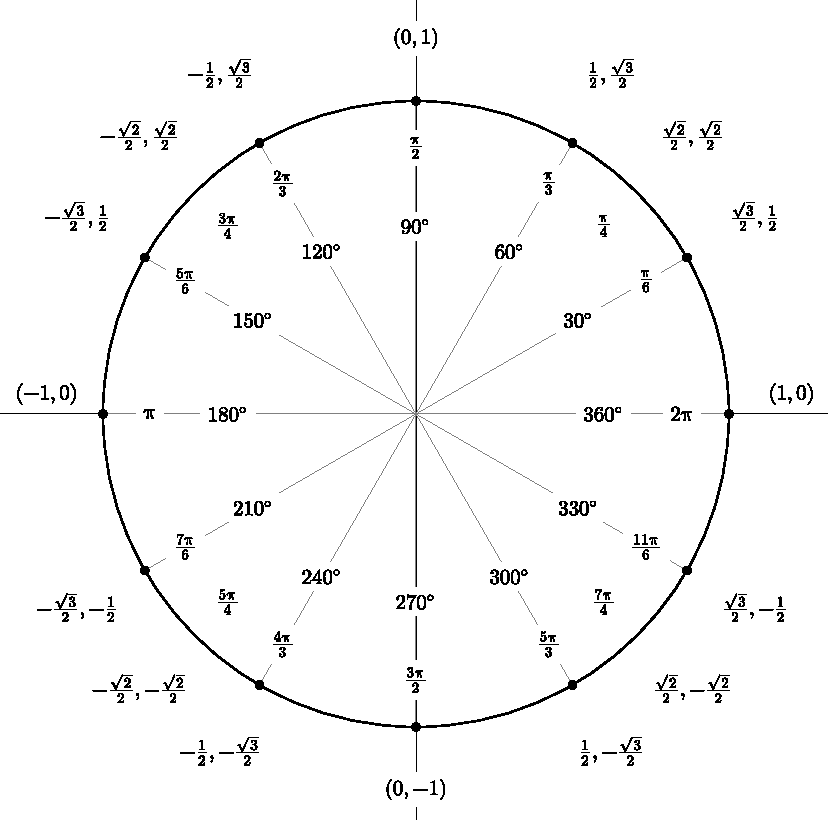
\includegraphics[width=\linewidth]{degrees_circle.pdf}
					  
					\definecolor{dg}{RGB}{12, 100, 0}
					\definecolor{db}{RGB}{12, 40, 150}
					\definecolor{dbt}{RGB}{20, 50, 160}
					\definecolor{dr}{RGB}{250, 0, 100}
					\definecolor{dark}{RGB}{100, 100, 100}
					\begin{tikzpicture}
						\begin{axis}%
							[grid=both,
								minor tick num=4,
								grid style={line width=.1pt, draw=gray!10},
								major grid style={line width=.2pt,draw=gray!50},
								axis lines=middle,
								enlargelimits={abs=0.4}
							]
							\addplot[domain=-1.3:1.3,samples=50,smooth,dg] {tan(deg(x))} node[right] {$\tan(x)$};
							\addplot[domain=-6.5:6.5,samples=50,smooth,db] {sin(deg(x))};
							\addplot[domain=-2*pi:2*pi,samples=50,smooth,dr] {cos(deg(x))};
							\node[dbt, above] at (axis cs:-4.6,1) {$\sin(x)$};
							\node[dr, above] at (axis cs:-3,-1.75) {$\cos(x)$};
							\draw[-, line width=0.2mm, dark] (pi,0) -- (pi,0.25) node[above] {$\pi$};
							\draw[-, line width=0.2mm, dark] (-pi,0) -- (-pi,0.25) node[above] {$-\pi$};
							\draw[-, line width=0.2mm, dark] (2*pi,0) -- (2*pi,0.25) node[above] {$2\pi$};    
							\draw[-, line width=0.2mm, dark] (-2*pi,0) -- (-2*pi,0.25) node[above] {$-2\pi$};
							\draw[-, line width=0.1mm, dark] (pi/2,0) -- (pi/2,0.25) node[above] {$\frac{\pi}{2}$};
							\draw[-, line width=0.1mm, dark] (-pi/2,0) -- (-pi/2,0.25) node[above] {$-\frac{\pi}{2}$};
						\end{axis}
					\end{tikzpicture}
					
				\end{center}
				
				\section{Tabellen}
				\subsection{Grenzwerte}
				\begin{center}
					\begin{tabularx}{\linewidth}{XX}
						\toprule
						$\limxi \frac{1}{x} = 0$                                   & $\limxi 1 + \frac{1}{x} = 1$             \\
						$\limxi e^x = \infty$                                      & $\limxn e^x = 0$                         \\
						$\limxi e^{-x} = 0$                                        & $\limxn e^{-x} = \infty$                 \\
						$\limxi \frac{e^x}{x^m} = \infty$                          & $\limxn xe^x = 0$                        \\
						$\limxi \ln(x) = \infty$                                   & $\limxo \ln(x) = -\infty$                \\
						$\limxi (1+x)^{\frac{1}{x}} = 1$                           & $\limxo (1+x)^{\frac{1}{x}} = e$         \\
						$\limxi (1+\frac{1}{x})^b = 1$                             & $\limxi n^{\frac{1}{n}} = 1$             \\
						$\lim_{x\to\pm\infty} (1 + \frac{1}{x})^x = e$             & $\limxi (1-\frac{1}{x})^x = \frac{1}{e}$ \\
						$\lim_{x\to\pm\infty} (1 + \frac{k}{x})^{mx} = e^{km}$     & $\limxi (\frac{x}{x+k})^x = e^{-k}$      \\
						$\limxo \frac{a^x -1}{x} = \ln(a), \newline \forall a > 0$ &                                          
						$\limxi x^a q^x = 0, \newline \forall 0 \le q < 1$ \\
					\end{tabularx}
					\begin{tabularx}{\linewidth}{XX}
						$\limxo \frac{\sin x}{x} = 1$                 & $\limxo \frac{\sin kx}{x} = k$     \\
						$\limxo \frac{1}{\cos x} = 1$                 & $\limxo \frac{\cos x -1}{x} = 0$   \\
						$\limxo \frac{\log 1 - x}{x} = -1$            & $\limxo x \log x = 0$              \\
						$\limxo \frac{1 - \cos x}{x^2} = \frac{1}{2}$ & $\limxo \frac{e^x-1}{x} = 1$       \\
						$\limxo \frac{x}{\arctan x} = 1$              & $\limxi \arctan x = \frac{\pi}{2}$ \\
						$\limxo \frac{e^{ax}-1}{x} = a$               & $\limxo \frac{\ln(x+1)}{x} = 1$    \\
						$\lim_{x\to 1} \frac{\ln(x)}{x-1} = 1$        & $\limxi \frac{\log(x)}{x^a} = 0$   \\
						$\limxi \sqrt[x]{x} = 1$                      & $\limxi \frac{2x}{2^x} = 0$        \\
						\multicolumn{2}{c}{$\lim_{x\to \infty} \left(\sqrt{ax^2+bx+c}-\sqrt{a}\cdot x \right) = \frac{b}{2\sqrt{a}}$} \\
						\bottomrule
					\end{tabularx}
				\end{center}
				
				\newpage
				\vfill\null
				
				\subsection{Ableitungen}
				\begin{center}
					% the c>{\centering\arraybackslash}X is a workaround to have a column fill up all space and still be centered
					\begin{tabularx}{\linewidth}{c>{\centering\arraybackslash}Xc}
						\toprule
						$\mathbf{F(x)}$                        & $\mathbf{f(x)}$          & $\mathbf{f'(x)}$               \\
						\midrule
						$\frac{x^{-a+1}}{-a+1}$                & $\frac{1}{x^a}$          & $\frac{-a}{x^{a+1}}$            \\
						$\frac{x^{a+1}}{a+1}$                  & $x^a \ (a \ne -1)$       & $a \cdot x^{a-1}$              \\
						$\frac{1}{k \ln(a)}a^{kx}$             & $a^{kx}$                 & $ka^{kx} \ln(a)$               \\
						$\ln |x|$                              & $\frac{1}{x}$            & $-\frac{1}{x^2}$               \\
						$\frac{2}{3}x^{3/2}$                   & $\sqrt{x}$               & $\frac{1}{2\sqrt{x}}$          \\
						$\frac{n}{n+1}x^{\frac{1}{n}+1}$       & $\sqrt[n]{x}$            & $\frac{1}{n}x^{\frac{1}{n}-1}$ \\
						$-\cos(x)$                             & $\sin(x)$                & $\cos(x)$                      \\
						$\sin(x)$                              & $\cos(x)$                & $-\sin(x)$                     \\
						$\frac{1}{2}(x-\frac{1}{2}\sin(2x))$   & $\sin^2(x)$              & $2 \sin(x)\cos(x)$             \\
						$\frac{1}{2}(x + \frac{1}{2}\sin(2x))$ & $\cos^2(x)$              & $-2\sin(x)\cos(x)$             \\
						\multirow{2}*{$-\ln|\cos(x)|$}         & \multirow{2}*{$\tan(x)$} & $\frac{1}{\cos^2(x)}$          \\
						                                       &                          & $1 + \tan^2(x)$                \\
						$\cosh(x)$                             & $\sinh(x)$               & $\cosh(x)$                     \\
						$\log(\cosh(x))$                       & $\tanh(x)$               & $\frac{1}{\cosh^2(x)}$         \\
						$\ln | \sin(x)|$                       & $\cot(x)$                & $-\frac{1}{\sin^2(x)}$         \\
						$\frac{1}{c} \cdot e^{cx}$             & $e^{cx}$                 & $c \cdot e^{cx}$               \\
						$x(\ln |x| - 1)$                       & $\ln |x|$                & $\frac{1}{x}$                  \\
						$\frac{1}{2}(\ln(x))^2$                & $\frac{\ln(x)}{x}$       & $\frac{1 - \ln(x)}{x^2}$       \\
						$\frac{x}{\ln(a)} (\ln|x| -1)$         & $\log_a |x|$             & $\frac{1}{\ln(a)x}$            \\
						\bottomrule
					\end{tabularx}
				\end{center}
				\subsection{Weitere Ableitungen}
				\begin{center}
					\begin{tabularx}{\linewidth}{>{\centering\arraybackslash}X>{\centering\arraybackslash}X}
						\toprule
						$\mathbf{F(x)}$                                     & $\mathbf{f(x)}$                          \\
						\midrule
						$\frac{1}{a\cdot (n+1)}(ax+b)^{n+1}$                & $(ax+b)^n$                               \\
						  
						$\arcsin(x)$                                        & $\frac{1}{\sqrt{1 - x^2}}$               \\
						$\arccos(x)$                                        & $\frac{-1}{\sqrt{1 - x^2}}$              \\
						$\arctan(x)$                                        & $\frac{1}{1 + x^2}$                      \\ 
						$\text{arcsinh}(x)$                                 & $\frac{1}{\sqrt{1 + x^2}}$               \\
						$\text{arccosh}(x) $                                & $\frac{1}{\sqrt{x^2 - 1}}$               \\
						$\text{arctanh}(x) $                                & $\frac{1}{1 - x^2}$                      \\ 
						$x^x \ (x > 0)$                                     & $x^x \cdot (1 + \ln x)$                  \\
						$\log_a|x|$                                         & $\frac{1}{x \ln a}=\log_a(e)\frac{1}{x}$ \\
						$\frac{(ax+b)^{n+2}}{a^2(n+1)(n+2)}$                & $\frac{(ax+b)^{n+1}}{a\cdot (n+1)}$      \\
						$\sqrt{1-x^2}+x\cdot \text{arcsin}(x)$              & $\arcsin(x)$                             \\
						$x\cdot \arccos(x)-\sqrt{1-x^2}$                    & $\arccos(x)$                             \\
						$x\cdot \arctan(x)-\frac{1}{2} \log(x^2+1)$         & $\arctan(x)$                             \\ 
						$x\cdot \text{arcsinh}(x)-\sqrt{x^2+1}$             & $\text{arcsinh}(x)$                      \\
						$x\cdot \text{arccosh}(x)-\sqrt{x^2-1}\sqrt{x^2+1}$ & $\text{arccosh}(x)$                      \\
						$\frac{1}{2} \log(1-x^2)+x\cdot \text{arctanh}(x)$  & $\text{arctanh}(x)$                      \\ 
						\bottomrule
					\end{tabularx}
				\end{center}
				\subsection{Integrale}
				\begin{center}
					\begin{tabularx}{\linewidth}{>{\centering\arraybackslash}X>{\centering\arraybackslash}X}
						\toprule
						$\mathbf{f(x)}$                      & $\mathbf{F(x)}$                                                  \\
						\midrule
						$\int f'(x) f(x) \dx$                & $\frac{1}{2}(f(x))^2$                                            \\
						$\int \frac{f'(x)}{f(x)} \dx$        & $\ln|f(x)|$                                                      \\
						$\int_{-\infty}^\infty e^{-x^2} \dx$ & $\sqrt{\pi}$                                                     \\
						$\int (ax+b)^n \dx$                  & $\frac{1}{a(n+1)}(ax+b)^{n+1}$                                   \\
						$\int x(ax+b)^n \dx$                 & $\frac{(ax+b)^{n+2}}{(n+2)a^2} - \frac{b(ax+b)^{n+1}}{(n+1)a^2}$ \\
						$\int (ax^p+b)^n x^{p-1} \dx$        & $\frac{(ax^p+b)^{n+1}}{ap(n+1)}$                                 \\
						$\int (ax^p + b)^{-1} x^{p-1} \dx$   & $\frac{1}{ap} \ln |ax^p + b|$                                    \\
						$\int \frac{ax+b}{cx+d} \dx$         & $\frac{ax}{c} - \frac{ad-bc}{c^2} \ln |cx +d|$                   \\
						$\int \frac{1}{x^2+a^2} \dx$         & $\frac{1}{a} \arctan \frac{x}{a}$                                \\
						$\int \frac{1}{x^2 - a^2} \dx$       & $\frac{1}{2a} \ln\left| \frac{x-a}{x+a} \right|$                 \\
						$\int \sqrt{a^2+x^2} \dx $           & $\frac{x}{2}f(x) + \frac{a^2}{2}\ln(x+f(x))$                     \\
						\bottomrule
					\end{tabularx}
				\end{center}
				
\end{document}
